\chapter{Análise das Lições Aprendidas Coletadas}

Após a seleção do conjunto de trabalhos primários dessa pesquisa (16 artigos científicos e 14 relatos de experiência), as lições aprendidas reportadas por eles foram devidamente mapeadas (coletadas) e categorizadas, de acordo com similaridades. Nesse capítulo encontra-se o resultado dessa categorização.

\section{Mapeamento e categorização}

As diversas lições aprendidas reportadas pela base da literatura científica e relatos de experiência foram separadas em categorias, por similaridade, para obter uma maior visibilidade do que foi encontrado. Alguns exemplos dessas categorias são: ``Apoio gerencial e dos clientes" e ``Aspectos técnicos e tecnológicos". Considerou-se a existência real de uma categoria quando pelo menos 6 trabalhos (20\% do material analisado) referenciavam alguma lição aprendida que se encaixasse naquela categoria.

A tabela \ref{tab:mapeamentoCategorias} apresentada abaixo relaciona as categorias criadas e, a cada categoria, estão relacionadas as referências dos artigos científicos (coluna 2) e relatos de experiência (coluna 3) que possuem lições aprendidas naquele contexto. Em seguida, a figura \ref{fig:categorias} é um gráfico que contabiliza a quantidade de trabalhos que referenciaram cada categoria de lições aprendidas.

\begin{table}[H]
	\centering
	\begin{tabularx}{\linewidth}{ | p{6cm} | X | X | }
		\hline 
		\textbf{Categorias} & \textbf{Artigos científicos} & \textbf{Relatos de experiência} \\ 
		\hline 
		Experiência, treinamento e aprendizado & \cite{Hajjdiab2011}, \cite{Block2011}, \cite{Adobe2012}, \cite{Cisco2011}, \cite{Lapham2012}, \cite{Eunha2012}, \cite{Claudia2013}, \cite{Asnawi2012}, \cite{Fitzgerald2013} & \cite{Stefano2013}, \cite{Rodrigues2013}, \cite{Bastos2013}, \cite{Maciel2013}, \cite{Karaj2013}, \cite{Piegas2012}, \cite{Vieira2013} \\ 
		\hline 
		Planejamento e gerenciamento de backlog & \cite{Hajjdiab2011}, \cite{Fitzgerald2013}, \cite{Block2011}, \cite{Adobe2012}, \cite{Bustard2013}, \cite{Korhonen2010}, \cite{Claudia2013} & \cite{Piegas2012}, \cite{Hui2013}, \cite{Parzinello2012} \\ 
		\hline 
		Apoio gerencial e dos clientes & \cite{Hajjdiab2011}, \cite{Cisco2011}, \cite{Claudia2013}, \cite{Arikpo2011} & \cite{Parzinello2012}, \cite{Stefano2013}, \cite{Bastos2013}, \cite{Maciel2013}, \cite{Srinath2012}, \cite{Piegas2012} \\ 
		\hline 
		Customização e adaptabilidade & \cite{Hajjdiab2011}, \cite{Block2011}, \cite{Asnawi2012}, \cite{Fitzgerald2013}, \cite{Bustard2013}, \cite{Microsoft2013}, \cite{Lapham2012}, \cite{Claudia2013}, \cite{Nokia2013} & \cite{Piegas2012}, \cite{Hui2013}, \cite{Rodrigues2013}, \cite{Bastos2013}, \cite{Maciel2013}, \cite{Ahmed2008}, \cite{Sahota2012}, \cite{Vieira2013} \\ 
		\hline 
		Confiança do time & \cite{Block2011}, \cite{Asnawi2012}, \cite{Claudia2013}, \cite{Nokia2013} & \cite{Parzinello2012}, \cite{Ahmed2008}, \cite{Piegas2012}, \cite{Bastos2013} \\ 
		\hline 
		Engajamento, comprometimento, disciplina e trabalho em equipe & \cite{Block2011}, \cite{Asnawi2012}, \cite{Lapham2012}, \cite{Microsoft2013}, \cite{Claudia2013}, \cite{Nokia2013}, \cite{Adobe2012}, \cite{Fitzgerald2013} & \cite{Piegas2012}, \cite{Parzinello2012}, \cite{Stefano2013}, \cite{Rodrigues2013}, \cite{Maciel2013}, \cite{Queiroz2013}, \cite{Bastos2013}, \cite{Ahmed2008} \\ 
		\hline 
		Aspectos técnicos e tecnológicos & \cite{Block2011}, \cite{Microsoft2013}, \cite{Korhonen2010}, \cite{Cisco2011}, \cite{Lapham2012}, \cite{Eunha2012}, \cite{Fitzgerald2013}, \cite{Arikpo2011}, \cite{Bustard2013}, \cite{Radha2012}, \cite{Nokia2013} & \cite{Piegas2012}, \cite{Queiroz2013}, \cite{Stefano2013}, \cite{Karaj2013} \\ 
		\hline 
		Compartilhamento de conhecimento & \cite{Asnawi2012}, \cite{Cisco2011}, \cite{Lapham2012}, \cite{Radha2012}, \cite{Eunha2012}, \cite{Ericsson2013} & \cite{Valerio2013}, \cite{Vieira2013}, \cite{Queiroz2013}, \cite{Bastos2013}, \cite{Maciel2013} \\ 
		\hline 
		Velocidade de entrega e produtividade & \cite{Adobe2012}, \cite{Fitzgerald2013}, \cite{Microsoft2013}, \cite{Cisco2011}, \cite{Korhonen2010}, \cite{Eunha2012}, \cite{Claudia2013} & \cite{Stefano2013}, \cite{Queiroz2013}, \cite{Maciel2013}, \cite{Hui2013}, \cite{Ahmed2008}, \cite{Piegas2012} \\ 
		\hline 
		Qualidade do produto final & \cite{Adobe2012}, \cite{Fitzgerald2013}, \cite{Bustard2013}, \cite{Lapham2012}, \cite{Eunha2012}, \cite{Claudia2013}, \cite{Korhonen2010} & \cite{Parzinello2012}, \cite{Maciel2013}, \cite{Ahmed2008} \\ 
		\hline 
		Tamanho da organização & \cite{Bustard2013}, \cite{Microsoft2013}, \cite{Claudia2013}, \cite{Korhonen2010}, \cite{Ericsson2013} & \cite{Maciel2013} \\ 
		\hline 
		Quebra de paradigma & \cite{Hajjdiab2011}, \cite{Block2011}, \cite{Korhonen2010}, \cite{Lapham2012}, \cite{Arikpo2011} & \cite{Stefano2013}, \cite{Bastos2013}, \cite{Maciel2013}, \cite{Parzinello2012}, \cite{Hui2013}, \cite{Ahmed2008}, \cite{Sahota2012} \\ 
		\hline 
		Comunicação remota & \cite{Adobe2012}, \cite{Microsoft2013}, \cite{Korhonen2010}, \cite{Radha2012} & \cite{Rodrigues2013}, \cite{Vieira2013}, \cite{Bastos2013}, \cite{Maciel2013} \\ 
		\hline 
		Cultura organizacional & \cite{Bustard2013}, \cite{Microsoft2013}, \cite{Claudia2013}, \cite{Nokia2013}, \cite{Eunha2012}, \cite{Fitzgerald2013} & \cite{Rodrigues2013}, \cite{Bastos2013}, \cite{Srinath2012}, \cite{Maciel2013}, \cite{Sahota2012} \\ 
		\hline 
	\caption{Mapeamento de categorias de lições aprendidas e suas respectivas referências}
	\label{tab:mapeamentoCategorias}
	\end{tabularx}
\end{table}

\begin{figure}[H]
	\centering
	\captionsetup{justification=centering,margin=2cm}
	\makebox[\textwidth]{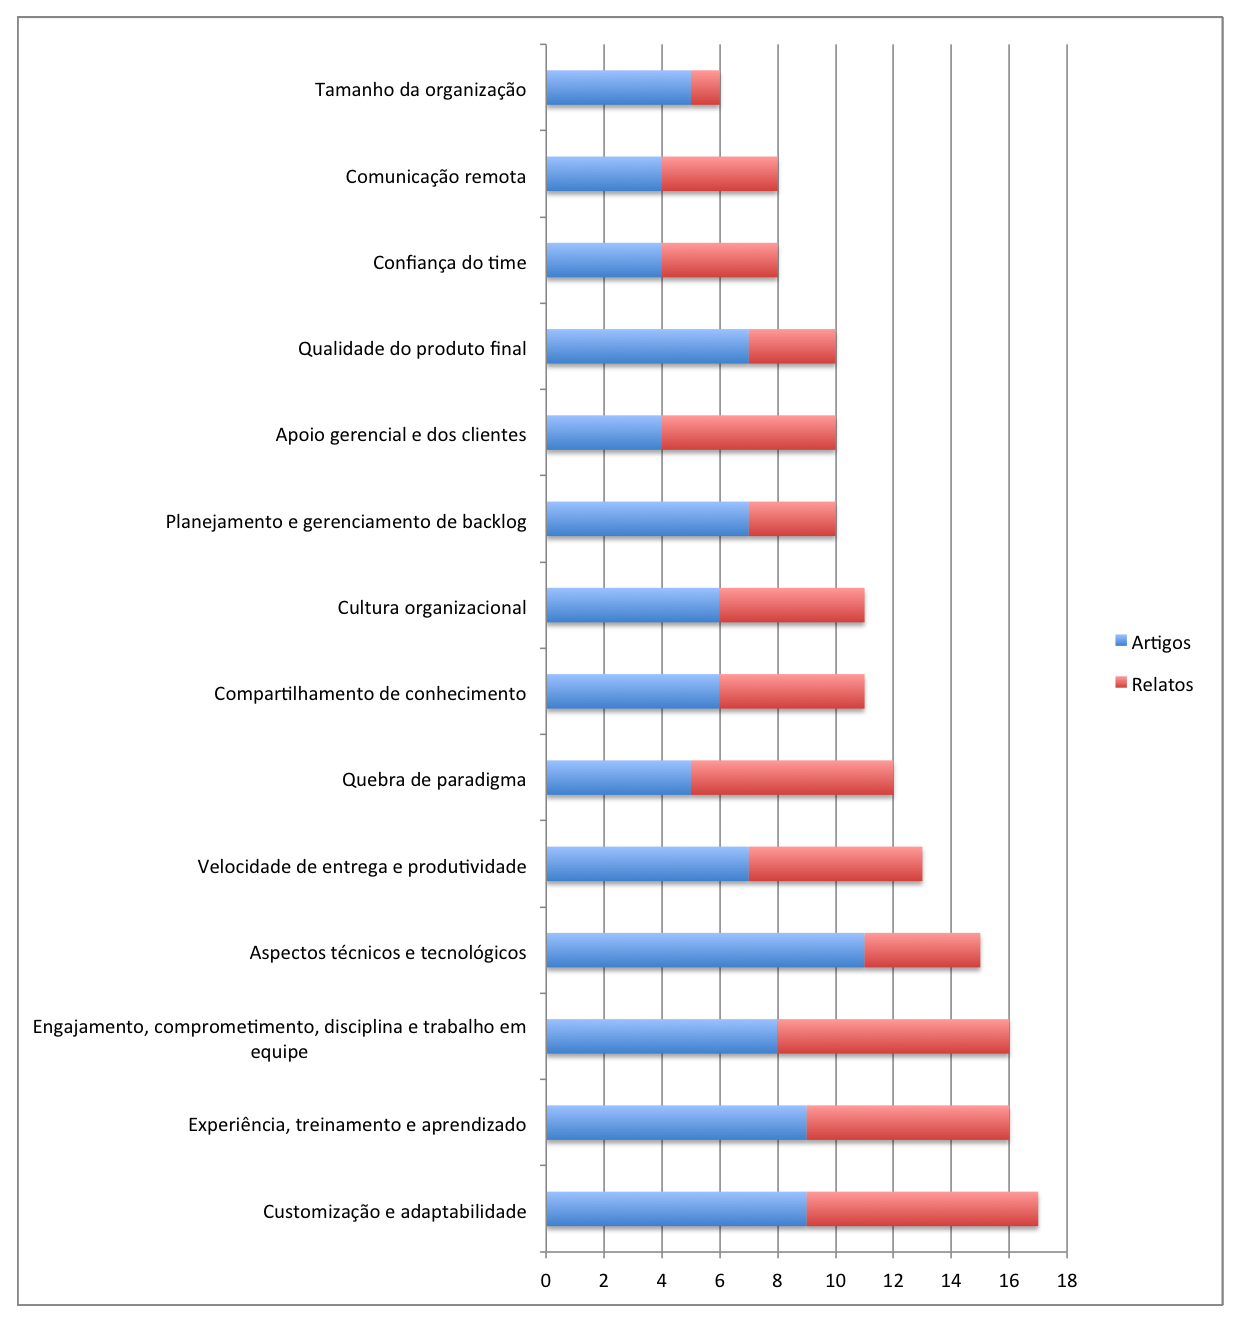
\includegraphics[width=\textwidth]{capitulos/las/figuras/categorias.eps}}
	\caption{Gráfico que contabiliza a quantidade de trabalhos que referenciaram cada categoria de lições aprendidas}
	\label{fig:categorias}
\end{figure}

\section{Análises das lições aprendidas}

Esta seção analisa as categorias com as respectivas lições aprendidas coletadas. Os percentuais de trabalhos que referenciaram cada categoria de lições aprendidas estão exibidos ao final de cada subseção correspondente. As áreas hachuradas em verde correspondem aos materiais que apontaram alguma lição aprendida daquela categoria.

\subsection{Experiência, treinamento e aprendizado}

\begin{table}[H]
	\centering
	\captionsetup{justification=centering}
	\begin{tabularx}{\linewidth}{ | X | p{5cm} | } \hline \textbf{Lições aprendidas} & \textbf{Referências} \\ \hline
		É muito difícil aventurar-se em Ágil sem um Agile Coach & \cite{Hajjdiab2011}, \cite{Block2011}, \cite{Adobe2012}, \cite{Cisco2011}, \cite{Lapham2012}, \cite{Eunha2012}, \cite{Claudia2013}, \cite{Stefano2013}, \cite{Rodrigues2013}, \cite{Bastos2013}, \cite{Maciel2013}, \cite{Karaj2013} \\ \hline
		Vivenciar um projeto-piloto é uma prática muito eficiente para se adquirir experiência & \cite{Hajjdiab2011}, \cite{Cisco2011}, \cite{Rodrigues2013}, \cite{Maciel2013} \\ \hline
		É preciso prática, não apenas estudo & \cite{Hajjdiab2011}, \cite{Asnawi2012}, \cite{Claudia2013}, \cite{Piegas2012}, \cite{Vieira2013} \\ \hline
		Trabalhar com equipes não-ágeis pode atrapalhar o andamento do projeto & \cite{Adobe2012}, \cite{Maciel2013} \\ \hline
	\caption{Lições aprendidas agrupadas na categoria ``Experiência, treinamento e aprendizado''}
	\end{tabularx}
\end{table}

Por muitos anos empresas de desenvolvimento de software adotaram o modelo cascata como forma de gerenciamento de projetos. O Manifesto Ágil \cite{agileManifesto}, ocorrido em 2001, modificou completamente a maneira de lidar com esse tipo de atividade.

Mudar bruscamente nunca é simples. Para que essa transição não seja tão dolorosa, uma tática muito popular entre as empresas é a contratação de um profissional experiente para servir como guia e treinar toda a equipe. Esse papel é essencial durante o processo de adoção ágil em qualquer organização \cite{Hajjdiab2011}. Outra maneira de se adquirir experiência de forma rápida e eficaz é através de um projeto-piloto. Power utilizou essa abordagem com o intuito de entender melhor como a empresa funcionava e tentar atacar os pontos mais críticos \cite{Cisco2011}.

Alguns pontos negativos também foram levantados nos trabalhos analisados. É preciso aprender com os próprios erros, não apenas realizar treinamentos \cite{Piegas2012}. E, de acordo com Green e Maciel, trabalhar com stakeholders que não são ágeis pode afetar negativamente o desempenho do time ágil, que trabalha em um ambiente menos burocrático e com um ciclo de feedback bem mais curto \cite{Adobe2012,Maciel2013}.

\begin{figure}[H]
	\centering
	\captionsetup{justification=centering}
	\makebox[\textwidth]{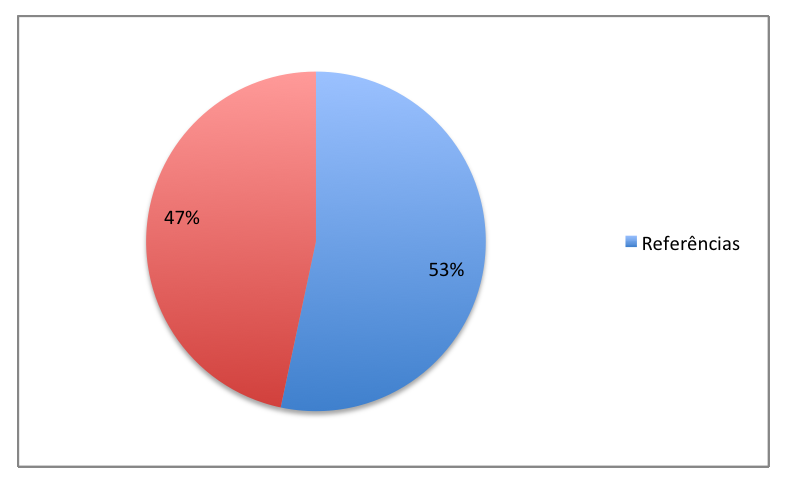
\includegraphics[width=0.8\textwidth]{capitulos/las/figuras/exp.eps}}
	\caption{Percentual de trabalhos que referenciaram lições aprendidas da categoria ``Experiência, treinamento e aprendizado"}
	\label{fig:exp}
\end{figure}

\subsection{Planejamento e gerenciamento de backlog}

\begin{table}[H]
	\centering
	\captionsetup{justification=centering}
	\begin{tabularx}{\linewidth}{ | X | p{5cm} | } \hline \textbf{Lições aprendidas} & \textbf{Referências} \\ \hline
		Planejar apenas quando necessário & \cite{Hajjdiab2011}, \cite{Fitzgerald2013}, \cite{Piegas2012}, \cite{Hui2013}, \cite{Parzinello2012} \\ \hline
		O processo de adoção em si precisa ser bem planejado & \cite{Hajjdiab2011} \\ \hline
		Priorizar o backlog é uma tarefa complicada para times inexperientes & \cite{Block2011} \\ \hline
		É difícil lidar com o aumento de escopo & \cite{Block2011} \\ \hline
		É preciso aprender a quebrar o backlog da forma correta & \cite{Adobe2012}, \cite{Hui2013}, \cite{Parzinello2012} \\ \hline
		A coleta e gerência de requisitos ocorre de forma bem diferente do habitual & \cite{Bustard2013}, \cite{Korhonen2010}, \cite{Claudia2013}, \cite{Piegas2012}, \cite{Hui2013} \\ \hline
	\caption{Lições aprendidas agrupadas na categoria `Planejamento e gerenciamento de backlog''}
	\end{tabularx}
\end{table}

Desenvolver de forma iterativa e incremental gera um grande impacto na forma de gerenciamento de projetos. Não é necessário planejar todas as etapas do processo, é difícil prever situações e cenários muito distantes. Planejar apenas o necessário, quando necessário, é um grande desafio para muitas empresas. Fitzgerald et al. relataram que tiveram que lidar com muitos problemas relacionados à granularidade no planejamento que Ágil propõe \cite{Fitzgerald2013}.

Todavia, não podemos confundir o processo de planejamento utilizado em projetos ágeis e o planejamento para se adotar Ágil. Dado que esta é uma grande mudança de paradigma, então é preciso ter cautela. Hajjdiab e Taleb aconselharam que esse processo deve ser bem planejado e que aconteça de forma gradual \cite{Hajjdiab2011}.

Outro ponto considerado desafiador por muitas organizações é o gerenciamento de backlog. Block relatou as dificuldades ao tentar priorizá-lo e impedir que ele crescesse além do comportado pela equipe \cite{Block2011}. Ainda com relação ao backlog, Green lembrou que um dos princípios primários do desenvolvimento ágil de software é o foco na entrega de pequenos incrementos de valor \cite{Adobe2012}. Isto pode até parecer simples à primeira impressão, porém dividir todo um conjunto de requisitos de um projeto em pequenas fatias independentes entre si e que agregam valor ao cliente não é algo trivial.

\begin{figure}[H]
	\centering
	\captionsetup{justification=centering}
	\makebox[\textwidth]{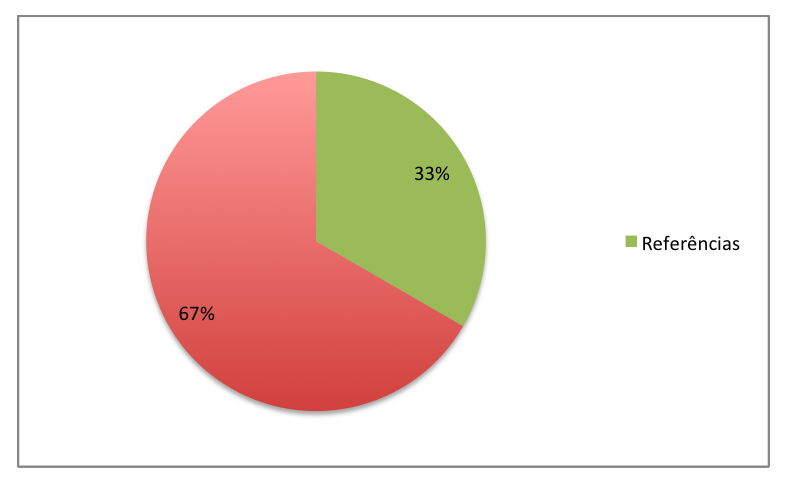
\includegraphics[width=0.8\textwidth]{capitulos/las/figuras/backlog.eps}}
	\caption{Percentual de trabalhos que referenciaram lições aprendidas da categoria ``Planejamento e gerenciamento de backlog"}
	\label{fig:backlog}
\end{figure}

\subsection{Apoio gerencial e dos clientes}

\begin{table}[H]
	\centering
	\captionsetup{justification=centering}
	\begin{tabularx}{\linewidth}{ | X | p{5cm} | } \hline \textbf{Lições aprendidas} & \textbf{Referências} \\ \hline
		Pressão por parte do alto escalão da empresa afeta negativamente no andamento do processo de adoção ágil & \cite{Hajjdiab2011}, \cite{Cisco2011}, \cite{Claudia2013}, \cite{Parzinello2012}, \cite{Stefano2013}, \cite{Bastos2013}, \cite{Maciel2013}, \cite{Srinath2012} \\ \hline
		O apoio do cliente é de suma importância para o sucesso do projeto & \cite{Arikpo2011}, \cite{Claudia2013}, \cite{Parzinello2012}, \cite{Stefano2013}, \cite{Maciel2013} \\ \hline
		É muito difícil contornar uma situação quando o cliente pressiona o tima para que se adote práticas waterfall & \cite{Claudia2013}, \cite{Piegas2012}, \cite{Srinath2012} \\ \hline
		É preciso ter liberdade ao se adotar Ágil & \cite{Piegas2012}, \cite{Stefano2013}, \cite{Maciel2013} \\ \hline
	\caption{Lições aprendidas agrupadas na categoria ``Apoio gerencial e dos cliente''}
	\end{tabularx}
\end{table}

Houve uma unanimidade quanto a este ponto. É preferível que todos os envolvidos em projetos de desenvolvimento de software que utilizam alguma metodologia ágil estejam alinhados com o processo. O apoio da gerência e dos clientes é fundamental para o bom desempenho da equipe.

Contudo, em muitos casos, apenas o apoio não é o suficiente. É preciso ter liberdade para se adotar Ágil de forma bem sucedida. Muitos relatos evidenciaram problemas com esse nível de alinhamento com os princípios ágeis de liberdade e auto-organização \cite{Piegas2012,Stefano2013,Maciel2013}.

\begin{figure}[H]
	\centering
	\captionsetup{justification=centering}
	\makebox[\textwidth]{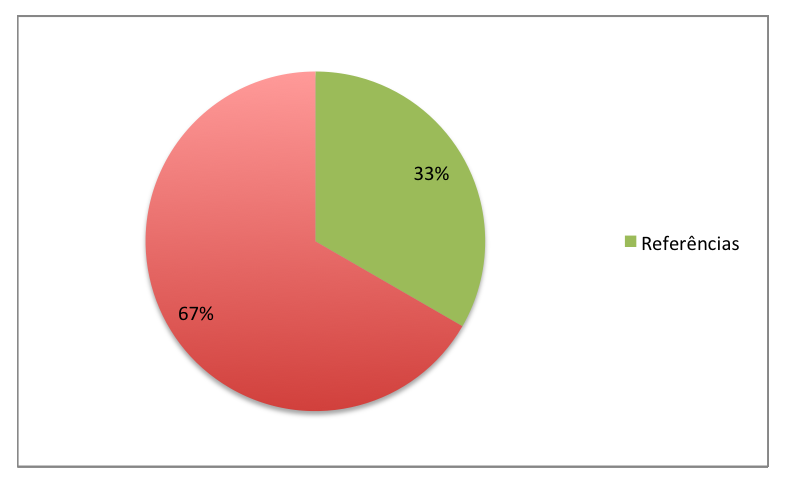
\includegraphics[width=0.8\textwidth]{capitulos/las/figuras/apoio.eps}}
	\caption{Percentual de trabalhos que referenciaram lições aprendidas da categoria ``Apoio gerencial e dos clientes"}
	\label{fig:apoio}
\end{figure}

\subsection{Customização e adaptabilidade}

\begin{table}[H]
	\centering
	\captionsetup{justification=centering}
	\begin{tabularx}{\linewidth}{ | X | p{5cm} | } \hline \textbf{Lições aprendidas} & \textbf{Referências} \\ \hline
		Ágil é customizável, não existem regras no seu processo de adoção & \cite{Hajjdiab2011}, \cite{Piegas2012}, \cite{Hui2013} \\ \hline
		Dar suporte para adaptabilidade é um problema não-trivial & \cite{Block2011}, \cite{Asnawi2012}, \cite{Fitzgerald2013}, \cite{Bustard2013}, \cite{Microsoft2013}, \cite{Lapham2012}, \cite{Claudia2013}, \cite{Nokia2013}, \cite{Rodrigues2013}, \cite{Bastos2013}, \cite{Maciel2013}, \cite{Hui2013}, \cite{Ahmed2008}, \cite{Sahota2012} \\ \hline
		Dificuldades na implantação de mudanças necessárias & \cite{Vieira2013}, \cite{Bastos2013}, \cite{Maciel2013}, \cite{Hui2013}, \cite{Sahota2012} \\ \hline
	\caption{Lições aprendidas agrupadas na categoria ``Customização e adaptabilidade''}
	\end{tabularx}
\end{table}

Um dos principais pilares do desenvolvimento ágil é encarar mudanças como bem-vindas. Todavia, atingir um nível de maturidade de tal forma que isto ocorra naturalmente é algo para se orgulhar. Muitos trabalhos relataram problemas para dar suporte a essa adaptabilidade. Em muitas situações, times encontraram dificuldades para implantar as mudanças necessárias para obter um melhor resultado final em seus projetos. Um exemplo claro desse fator é o demonstrado por Fitzgerald et al. Segundo seus autores, ambientes regulados e métodos ágeis são frequentemente vistos como fundamentalmente incompatíveis, o que causa uma série de problemas de adaptabilidade \cite{Fitzgerald2013}.

Outro ponto relevante abordado por alguns trabalhos é o quanto Ágil pode ser customizável. Não exite um conjunto pré-definido de regras que devem ser seguidas à risca por aqueles que querem ser ágeis. Ágil é flexível. Segundo Hajjdiab e Taleb, um dos principais benefícios do desenvolvimento ágil é a sua capacidade de ser personalizado baseado na cultura e no ambiente da organização que o está adotando \cite{Hajjdiab2011}.

\begin{figure}[H]
	\centering
	\captionsetup{justification=centering}
	\makebox[\textwidth]{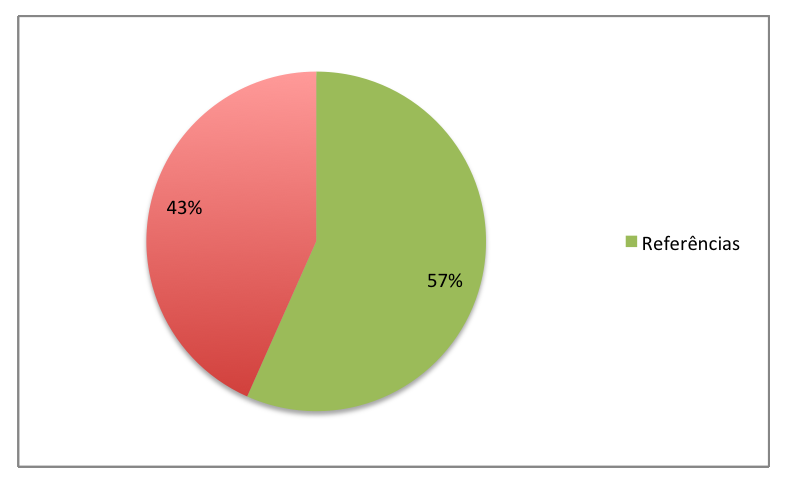
\includegraphics[width=0.8\textwidth]{capitulos/las/figuras/adaptabilidade.eps}}
	\caption{Percentual de trabalhos que referenciaram lições aprendidas da categoria ``Customização e adaptabilidade"}
	\label{fig:adaptabilidade}
\end{figure}

\subsection{Confiança do time}

\begin{table}[H]
	\centering
	\captionsetup{justification=centering}
	\begin{tabularx}{\linewidth}{ | X | p{5cm} | } \hline \textbf{Lições aprendidas} & \textbf{Referências} \\ \hline
		Entregar mais e entregar valor  ajuda a manter o time confiante & \cite{Block2011}, \cite{Asnawi2012}, \cite{Parzinello2012} \\ \hline
		Utilizar métodos ágeis ajuda a manter elevado o ânimo do time & \cite{Asnawi2012}, \cite{Claudia2013}, \cite{Nokia2013}, \cite{Ahmed2008} \\ \hline
		A manutenção da confiança das partes envolvidas se mostrou comprometida com o uso de metodologias ágeis & \cite{Nokia2013}, \cite{Piegas2012}, \cite{Bastos2013} \\ \hline
	\caption{Lições aprendidas agrupadas na categoria ``Confiança do time''}
	\end{tabularx}
\end{table}

Antes de analisar esse ponto, é preciso ter em mente que Ágil não é (nem nunca quis ser) a solução dos problemas causados por processos orientados a planejamento. Não existe solução mágica quando o assunto é desenvolvimento de software \cite{Piegas2012,Microsoft2013}.

Houve uma grande divergência com relação ao impacto causado por Ágil na confiança dos envolvidos. Enquanto vários trabalhos apontaram que o uso de métodos ágeis contribui com a manutenção do moral elevado do time, outros apontaram exatamente o oposto.

De acordo com Asnawi et al., o fato de Ágil proporcionar uma maior frequência de entregas de pedaços de software que agregam valor ao cliente torna o desenvolvimento do projeto mais prazeroso, menos estressante \cite{Asnawi2012}. Em contrapartida, Korhonen relatou que, em certos casos, é desmotivador trabalhar em um cenário onde não há uma visão clara do que está por vir a longo prazo \cite{Nokia2013}.

\begin{figure}[H]
	\centering
	\captionsetup{justification=centering}
	\makebox[\textwidth]{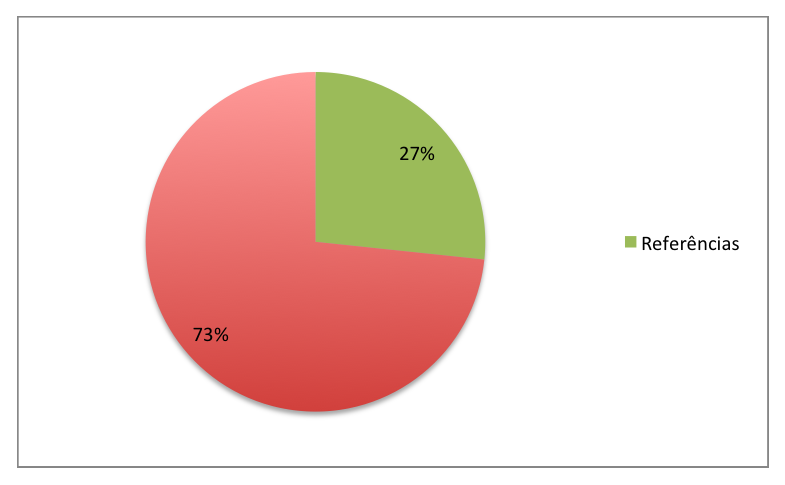
\includegraphics[width=0.8\textwidth]{capitulos/las/figuras/confianca.eps}}
	\caption{Percentual de trabalhos que referenciaram lições aprendidas da categoria ``Confiança do time"}
	\label{fig:confianca}
\end{figure}

\subsection{Engajamento, comprometimento, disciplina e trabalho em equipe}

\begin{table}[H]
	\centering
	\captionsetup{justification=centering}
	\begin{tabularx}{\linewidth}{ | X | p{5cm} | } \hline \textbf{Lições aprendidas} & \textbf{Referências} \\ \hline
		É difícil encontrar pessoas que trabalham bem em equipe & \cite{Block2011} \\ \hline
		É muito importante ter o PO próximo ou, se possível, como membro ativo do time, envolvido em todas as etapas do processo & \cite{Block2011}, \cite{Asnawi2012}, \cite{Lapham2012}, \cite{Microsoft2013}, \cite{Claudia2013}, \cite{Piegas2012}, \cite{Parzinello2012}, \cite{Stefano2013}, \cite{Rodrigues2013}, \cite{Maciel2013} \\ \hline
		Falta de ownership no projeto & \cite{Block2011}, \cite{Nokia2013}, \cite{Queiroz2013} \\ \hline
		O envolvimento dos desenvolvedores dentro do processo é extremamente importante & \cite{Asnawi2012}, \cite{Adobe2012}, \cite{Fitzgerald2013}, \cite{Lapham2012}, \cite{Microsoft2013}, \cite{Claudia2013}, \cite{Stefano2013}, \cite{Bastos2013}, \cite{Maciel2013}, \cite{Ahmed2008} \\ \hline
		Para projetos ágeis serem bem sucedidos, é preciso disciplina & \cite{Parzinello2012} \\ \hline
	\caption{Lições aprendidas agrupadas na categoria ``Engajamento, comprometimento, disciplina e trabalho em equipe''}
	\end{tabularx}
\end{table}

\nomenclature{PO}{Product Owner}%

Para que a construção e entrega de um software sejam bem sucedidas, é preciso esforço de diversos profissionais: desenvolvedores, analistas de qualidade, analistas de negócio, product owners, etc. Ficou bem claro que, para as empresas de desenvolvimento de software analisadas, todos os stakeholders precisam estar fortemente envolvidos em todas as etapas do processo de construção do produto. Contudo, um desafio visualizado através dos artigos e relatos foi o de manter o PO engajado. Um exemplo citado por Block é a dificuldade em manter o cliente próximo para que ele defina novas funcionalidades e priorize o backlog \cite{Block2011}. Situações como esta podem prejudicar consideravelmente o resultado final do projeto, causando frustração para ambos os lados.

Outro ponto pouco citado, porém relevante, é a questão da disciplina em projetos ágeis. Dado que, na teoria, deveríamos ter um ambiente menos controlado e com times auto-organizáveis. Disciplina é uma característica que precisa surgir naturalmente, visto que não existe um plano detalhado a ser seguido. Dalcin e Parzinello afirmaram que não se deve culpar o SCRUM (umas das metodologias ágeis mais populares) por sua falta de disciplina \cite{Parzinello2012}.

\begin{figure}[H]
	\centering
	\captionsetup{justification=centering}
	\makebox[\textwidth]{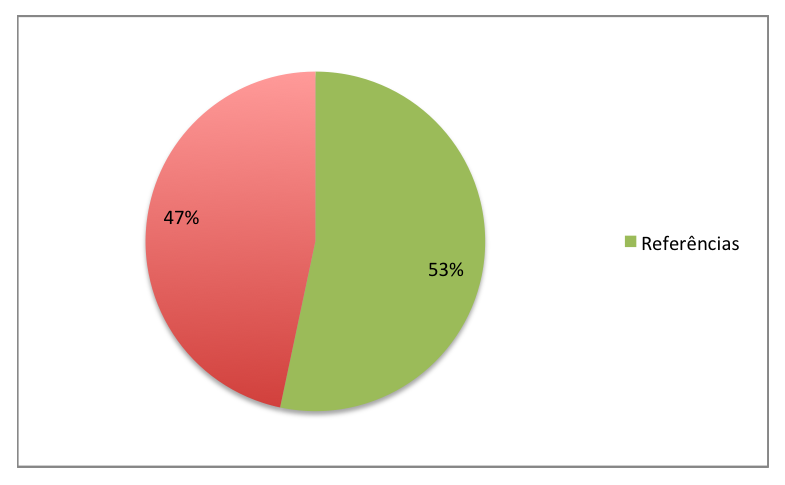
\includegraphics[width=0.8\textwidth]{capitulos/las/figuras/comprometimento.eps}}
	\caption{Percentual de trabalhos que referenciaram lições aprendidas da categoria ``Engajamento, comprometimento, disciplina e trabalho em equipe"}
	\label{fig:comprometimento}
\end{figure}

\subsection{Aspectos técnicos e tecnológicos}

\begin{table}[H]
	\centering
	\captionsetup{justification=centering}
	\begin{tabularx}{\linewidth}{ | X | p{5cm} | } \hline \textbf{Lições aprendidas} & \textbf{Referências} \\ \hline
		Utilizar Ágil em um projeto com código legado se mostrou desafiador & \cite{Block2011} \\ \hline
		Integração contínua, automação de build e testes automatizados promovem ganhos muito vantajosos & \cite{Block2011}, \cite{Microsoft2013}, \cite{Korhonen2010}, \cite{Cisco2011}, \cite{Lapham2012}, \cite{Eunha2012} \\ \hline
		É necessário o suporte de boas ferramentas & \cite{Fitzgerald2013}, \cite{Microsoft2013}, \cite{Arikpo2011} \\ \hline
		A atividade de design arquitetural se mostrou desafiadora & \cite{Bustard2013}, \cite{Radha2012}, \cite{Piegas2012} \\ \hline
		Ágil promove uma melhor manutenibilidade do código & \cite{Bustard2013} \\ \hline
		Infra-estruturas virtualizadas proporcionam a flexibilidade necessária para muitos projetos ágeis & \cite{Radha2012} \\ \hline
		Ágil promove uma pior manutenibilidade do código & \cite{Nokia2013}, \cite{Queiroz2013} \\ \hline
		Em certos casos há resistência por parte do cliente para utilizar o produto construído & \cite{Stefano2013} \\ \hline
	\caption{Lições aprendidas agrupadas na categoria ``Aspectos técnicos e tecnológicos''}
	\end{tabularx}
\end{table}

Aspectos técnicos são muito peculiares, variam de projeto para projeto. Por conta disso, várias lições aprendidas referentes a esses aspectos foram coletadas. Todavia, um padrão observado é que muitas fontes fizeram alusão a uma prática relativamente comum em projetos ágeis: a implantação de um servidor de integração contínua. Pode-se usufruir de muitos benefícios a partir dessa prática, como, por exemplo, a automação de testes e deploy automático de código. Para Block, essas mudanças técnicas tiveram um papel fundamental no nível de sucesso que puderam conquistar com práticas ágeis \cite{Block2011}.

Não planejar todos os detalhes de um projeto antes do seu início causa uma série de impactos no seu fluxo de atividades. Uma área bastante afetada por essa característica de Ágil é o design arquitetural. Diversos relatos afirmaram ter enfrentado muitos problemas com isso. Segundo Bustard et al., algumas empresas consideraram Ágil um retrocesso nesse aspecto \cite{Bustard2013}.

A manutenibilidade de código foi o ponto polêmico dessa categoria. Korhonen relatou passar por dificuldades em gerenciar muitas pessoas modificando o mesmo código simultaneamente \cite{Nokia2013}, enquanto Bustard et al. mostraram que, em diversas empresas, a melhoria na qualidade e manutenibilidade do código foi um dos principais ganhos com o uso de metodologias ágeis \cite{Bustard2013}.

\begin{figure}[H]
	\centering
	\captionsetup{justification=centering}
	\makebox[\textwidth]{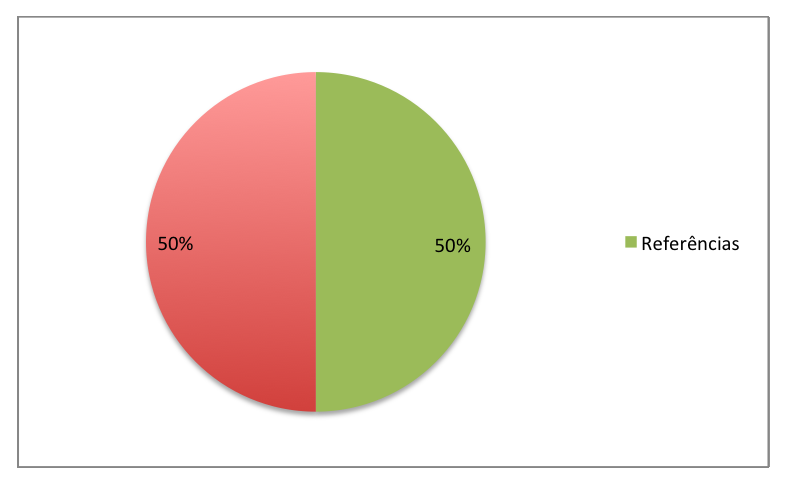
\includegraphics[width=0.8\textwidth]{capitulos/las/figuras/tech.eps}}
	\caption{Percentual de trabalhos que referenciaram lições aprendidas da categoria ``Aspectos técnicos e tecnológicos"}
	\label{fig:tech}
\end{figure}

\subsection{Compartilhamento de conhecimento}

\begin{table}[H]
	\centering
	\captionsetup{justification=centering}
	\begin{tabularx}{\linewidth}{ | X | p{5cm} | } \hline \textbf{Lições aprendidas} & \textbf{Referências} \\ \hline
		Compartilhar conhecimento e experiências é crucial para o sucesso de projetos ágeis & \cite{Asnawi2012}, \cite{Cisco2011}, \cite{Lapham2012}, \cite{Radha2012}, \cite{Eunha2012}, \cite{Valerio2013}, \cite{Vieira2013}, \cite{Queiroz2013}, \cite{Bastos2013}, \cite{Maciel2013} \\ \hline
		O ambiente com uma cultura ágil favorece o compartilhamento de conhecimento & \cite{Ericsson2013} \\ \hline
	\caption{Lições aprendidas agrupadas na categoria ``Compartilhamento de conhecimento''}
	\end{tabularx}
\end{table}

Segundo o Manifesto Ágil \cite{agileManifesto}, indivíduos e interações entre eles devem ser mais valorizados que processos e ferramentas. Outro ponto citado pelo Manifesto é que o método mais eficiente e eficaz de transmitir informações para e por um time de desenvolvimento é através de uma conversa cara a cara. Lagerberg et al. perceberam que Ágil de fato proporciona um ambiente que favorece essa troca de informações, tanto entre projetos como entre pessoas de um mesmo projeto \cite{Ericsson2013}. Muitos trabalhos evidenciaram a importância do compartilhamento de conhecimento para o sucesso de projetos ágeis. Nenhum se opôs a isso.

\begin{figure}[H]
	\centering
	\captionsetup{justification=centering}
	\makebox[\textwidth]{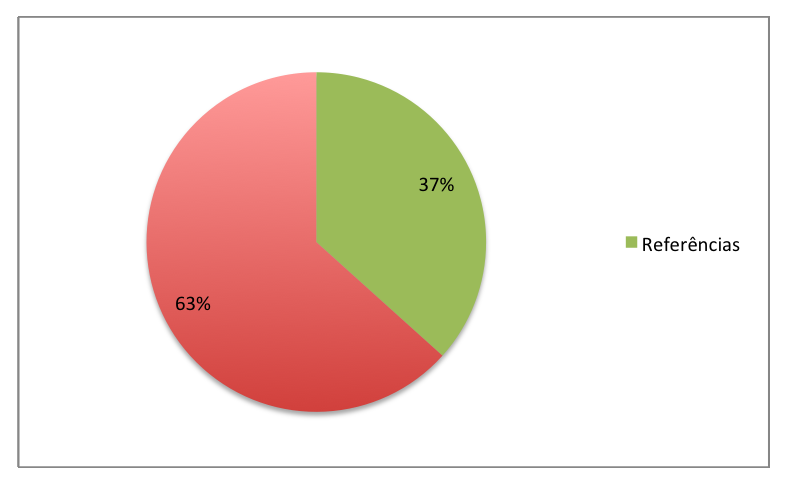
\includegraphics[width=0.8\textwidth]{capitulos/las/figuras/conhecimento.eps}}
	\caption{Percentual de trabalhos que referenciaram lições aprendidas da categoria ``Compartilhamento de conhecimento"}
	\label{fig:conhecimento}
\end{figure}

\subsection{Velocidade de entrega e produtividade}

\begin{table}[H]
	\centering
	\captionsetup{justification=centering}
	\begin{tabularx}{\linewidth}{ | X | p{5cm} | } \hline \textbf{Lições aprendidas} & \textbf{Referências} \\ \hline
		Há um aumento na velocidade/frequência de entrega com Ágil & \cite{Adobe2012}, \cite{Fitzgerald2013}, \cite{Microsoft2013}, \cite{Cisco2011}, \cite{Korhonen2010}, \cite{Eunha2012}, \cite{Claudia2013}, \cite{Stefano2013}, \cite{Queiroz2013}, \cite{Maciel2013}, \cite{Hui2013}, \cite{Ahmed2008} \\ \hline
		Defeitos são corrigidos mais rapidamente & \cite{Microsoft2013}, \cite{Korhonen2010} \\ \hline
		A velocidade do time é variável & \cite{Piegas2012} \\ \hline
	\caption{Lições aprendidas agrupadas na categoria ``Velocidade de entrega e produtividade''}
	\end{tabularx}
\end{table}

A maneira como projetos ágeis são estruturados (iterativos e incrementais) proporciona uma maior quantidade de entregas ao longo do tempo. Esse foi um ponto abordado em diversos trabalhos. No caso de Fitzgerald et al., as releases frequentes e a ativa sincronização com  seus clientes fizeram com que solicitações pudessem ser resolvidas num tempo, em média, menor que cinco semanas, fator que contribuiu para uma maior satisfação do cliente \cite{Fitzgerald2013}. Segundo a pesquisa feita por Claudia et al., o aumento da produtividade e o ganho na capacidade de gerenciamento de mudança de prioridades foram os benefícios mais facilmente percebidos ao se adotar Ágil \cite{Claudia2013}.

Um fator bastante relevante foi apontado por Murphy et al. e Korhonen \cite{Microsoft2013,Korhonen2010}. Segundo estes artigos, utilizar Ágil não diminui a quantidade de defeitos encontrados no decorrer do projeto. Contudo, o tempo necessário para a correção dos mesmos diminui drasticamente. Comparando o tempo necessário para a resolução de defeitos em projetos ágeis com projetos não-ágeis, cerca de 80\% dos defeitos encontrados demoraram mais a serem resolvidos em projetos não-ágeis \cite{Korhonen2010}.

Outra lição aprendida observada pela pesquisa foi com relação à variação de velocidade de times ágeis. É natural que, após um certo tempo, times ágeis andem a passos constantes, contudo, de acordo com Piegas e Peres, ocorrer uma variação de velocidade é comum, pois não necessariamente todas as sprints possuem a mesma tonalidade \cite{Piegas2012}.

\begin{figure}[H]
	\centering
	\captionsetup{justification=centering}
	\makebox[\textwidth]{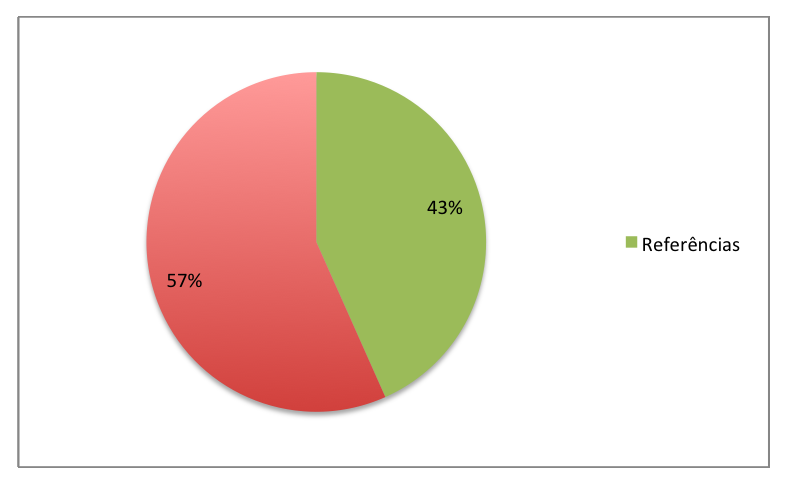
\includegraphics[width=0.8\textwidth]{capitulos/las/figuras/produtividade.eps}}
	\caption{Percentual de trabalhos que referenciaram lições aprendidas da categoria ``Velocidade de entrega e produtividade"}
	\label{fig:produtividade}
\end{figure}

\subsection{Qualidade do produto final}

\begin{table}[H]
	\centering
	\captionsetup{justification=centering}
	\begin{tabularx}{\linewidth}{ | X | p{5cm} | } \hline \textbf{Lições aprendidas} & \textbf{Referências} \\ \hline
		A melhoria na qualidade e valor agregado do produto é notória ao se desenvolver utilizando Ágil & \cite{Adobe2012}, \cite{Fitzgerald2013}, \cite{Bustard2013}, \cite{Lapham2012}, \cite{Eunha2012}, \cite{Claudia2013}, \cite{Parzinello2012}, \cite{Maciel2013}, \cite{Ahmed2008} \\ \hline
		Testar a aplicação durante o seu desenvolvimento reduz riscos & \cite{Korhonen2010}, \cite{Lapham2012}, \cite{Eunha2012}, \cite{Parzinello2012}, \cite{Ahmed2008} \\ \hline
	\caption{Lições aprendidas agrupadas na categoria ``Qualidade do produto final}
	\end{tabularx}
\end{table}

O ganho de qualidade com o uso de metodologias ágeis foi outra lição aprendida bastante mencionada. Algumas práticas adotadas por Green foram fundamentais para a obtenção desse ganho: divisão do trabalho em pequenas fatias que agregam valor ao cliente, definição de critérios de aceitação para cada uma dessas pequenas fatias e criação de times multifuncionais com experiência em testes e engenharia de software. Esse ganho de qualidade não é apenas percebido pelo time, mas também pelo cliente \cite{Adobe2012}.

O motivo desse ganho de qualidade, para muitos trabalhos, é decorrente da maneira de se testar aplicações em projetos ágeis. Automatizar o processo de testes, além de trazer muita segurança para o processo de desenvolvimento do software, propicia um curto ciclo de feedback.

\begin{figure}[H]
	\centering
	\captionsetup{justification=centering}
	\makebox[\textwidth]{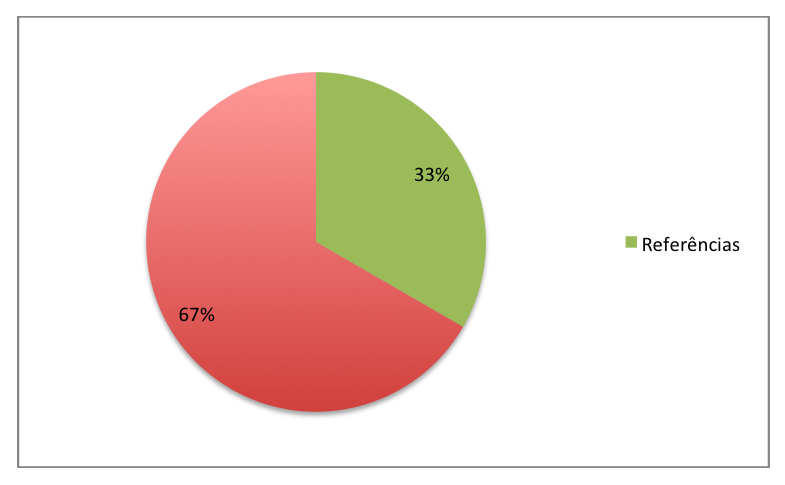
\includegraphics[width=0.8\textwidth]{capitulos/las/figuras/qualidade.eps}}
	\caption{Percentual de trabalhos que referenciaram lições aprendidas da categoria ``Qualidade do produto final"}
	\label{fig:qualidade}
\end{figure}

\subsection{Tamanho da organização}

\begin{table}[H]
	\centering
	\captionsetup{justification=centering}
	\begin{tabularx}{\linewidth}{ | X | p{5cm} | } \hline \textbf{Lições aprendidas} & \textbf{Referências} \\ \hline
		Pequenas empresas conseguem obter benefícios mais facilmente ao adotar Ágil & \cite{Bustard2013} \\ \hline
		Escalar Ágil para empresas ou projetos maiores é complicado, porém não é impossível & \cite{Microsoft2013}, \cite{Claudia2013}, \cite{Korhonen2010}, \cite{Maciel2013} \\ \hline
		É possível implementar Ágil parcialmente & \cite{Ericsson2013} \\ \hline
	\caption{Lições aprendidas agrupadas na categoria ``Tamanho da organização}
	\end{tabularx}
\end{table}

O Manifesto Ágil não faz menção a restrições com relação ao tamanho da empresa que deve ou não adotar Ágil. Contudo, alguns trabalhos relataram ter passado por muitas dificuldades devido ao porte da organização. Para Bustard et al., empresas menores e mais horizontais conseguem obter benefícios muito mais facilmente \cite{Bustard2013}. Vários trabalhadores consultados por Murphy et al. apontaram que escalabilidade pode ser um problema ao se tentar praticar Ágil \cite{Microsoft2013}.

\begin{figure}[H]
	\centering
	\captionsetup{justification=centering}
	\makebox[\textwidth]{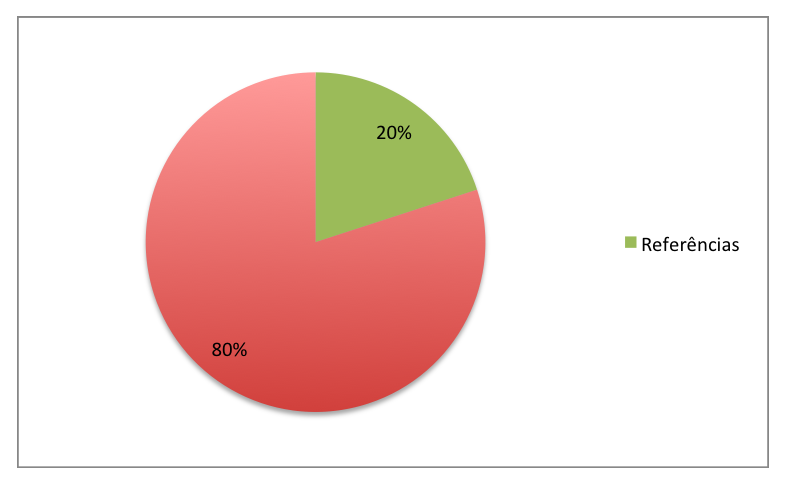
\includegraphics[width=0.8\textwidth]{capitulos/las/figuras/tamanho.eps}}
	\caption{Percentual de trabalhos que referenciaram lições aprendidas da categoria ``Tamanho da organização"}
	\label{fig:tamanho}
\end{figure}

\subsection{Quebra de paradigma}

\begin{table}[H]
	\centering
	\captionsetup{justification=centering}
	\begin{tabularx}{\linewidth}{ | X | p{5cm} | } \hline \textbf{Lições aprendidas} & \textbf{Referências} \\ \hline
		É difícil lidar com a quebra de paradigma para a implementação de Ágil & \cite{Hajjdiab2011}, \cite{Block2011}, \cite{Korhonen2010}, \cite{Lapham2012}, \cite{Arikpo2011}, \cite{Stefano2013}, \cite{Bastos2013}, \cite{Maciel2013} \\ \hline
		A maneira de gerenciar/implementar os testes de softwares construídos em projetos ágeis é desafiadora & \cite{Korhonen2010} \\ \hline
		Colocar princípios acima de práticas & \cite{Maciel2013}, \cite{Parzinello2012}, \cite{Hui2013}, \cite{Ahmed2008}, \cite{Sahota2012} \\ \hline
	\caption{Lições aprendidas agrupadas na categoria ``Quebra de paradigma''}
	\end{tabularx}
\end{table}

Muitas empresas tentam adotar Ágil com a finalidade de apenas usufruir de seus benefícios, contudo, não param para refletir que são fundamentalmente incompatíveis com muitos dos princípios ágeis \cite{Lapham2012,Bastos2013}. Fazer com que a alta gerência compreenda que é necessário modificar a essência da organização ao invés de simplesmente adotar um conjunto de práticas é algo bastante desafiador. Muitos dos trabalhos analisados mostraram ter apresentado problemas com isso. É preciso colocar os princípios acima das práticas \cite{Maciel2013}.

Uma das maiores quebras de paradigma está relacionada ao processo de testes ágeis \cite{Korhonen2010}. Passar a testar a aplicação durante o seu processo de desenvolvimento requer muita disciplina e capacidade técnica de implementação.

\begin{figure}[H]
	\centering
	\captionsetup{justification=centering}
	\makebox[\textwidth]{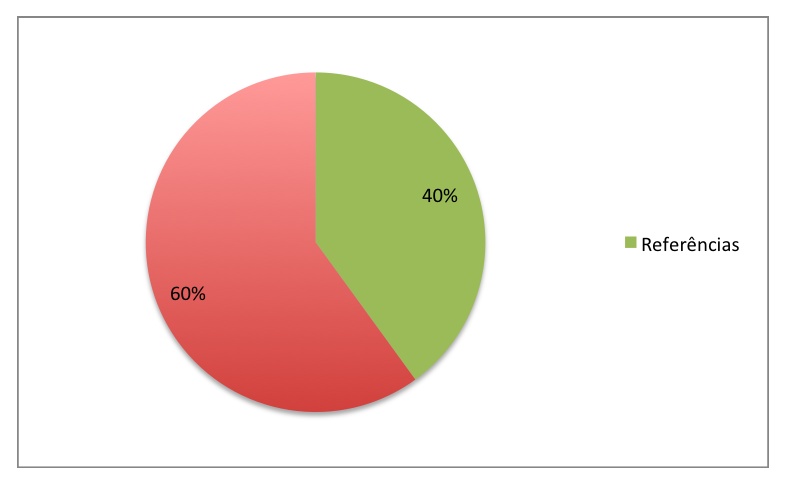
\includegraphics[width=0.8\textwidth]{capitulos/las/figuras/paradigma.eps}}
	\caption{Percentual de trabalhos que referenciaram lições aprendidas da categoria ``Quebra de paradigma"}
	\label{fig:paradigma}
\end{figure}

\subsection{Comunicação remota}

\begin{table}[H]
	\centering
	\captionsetup{justification=centering}
	\begin{tabularx}{\linewidth}{ | X | p{5cm} | } \hline \textbf{Lições aprendidas} & \textbf{Referências} \\ \hline
		Coordernar atividades com times distribuídos é algo bastante desafiador & \cite{Adobe2012}, \cite{Microsoft2013}, \cite{Korhonen2010}, \cite{Radha2012}, \cite{Rodrigues2013}, \cite{Vieira2013}, \cite{Bastos2013}, \cite{Maciel2013} \\ \hline
		Sincronizar boards virtual e real não é uma tarefa fácil & \cite{Vieira2013} \\ \hline
		Dificuldade ao trabalhar com equipes externas de testes & \cite{Bastos2013} \\ \hline
	\caption{Lições aprendidas agrupadas na categoria ``Comunicação remota''}
	\end{tabularx}
\end{table}

Dividir para conquistar é uma estratégia bastante antiga e que, muitas vezes, também se aplica à Ágil. Entretanto, muitas empresas se mostraram incapazes de gerenciar suas atividades diárias ao utilizar desenvolvimento distribuído de software. Atividades corriqueiras como trabalhar com equipes externas de testes \cite{Bastos2013} e sincronização de boards \cite{Vieira2013} se mostraram problemáticas.

Isso não ocorreu apenas com empresas pequenas e inexperientes. Grandes companhias também passaram por problemas dessa natureza. Uma pesquisa executada na Adobe relatou que, ao adotar uma abordagem distribuída em um de seus projetos, atividades corriqueiras como Sprint Planning, Daily Scrum, Sprint Review e Sprint Retrospective se mostraram desafiadoras \cite{Adobe2012}.

\begin{figure}[H]
	\centering
	\captionsetup{justification=centering}
	\makebox[\textwidth]{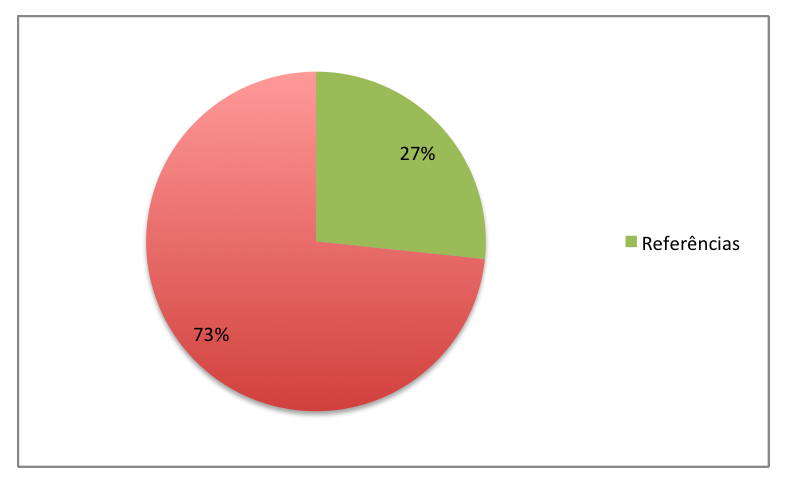
\includegraphics[width=0.8\textwidth]{capitulos/las/figuras/comunicacao.eps}}
	\caption{Percentual de trabalhos que referenciaram lições aprendidas da categoria ``Comunicação remota"}
	\label{fig:comunicacao}
\end{figure}

\subsection{Cultura organizacional}

\begin{table}[H]
	\centering
	\captionsetup{justification=centering}
	\begin{tabularx}{\linewidth}{ | X | p{5cm} | } \hline \textbf{Lições aprendidas} & \textbf{Referências} \\ \hline
		Métodos ágeis e ambientes altamente controlados são culturalmente incompatíveis & \cite{Fitzgerald2013} \\ \hline
		Empresas que discordam de princípios ágeis tendem a falhar caso tentem implantar tais métodos & \cite{Bustard2013}, \cite{Microsoft2013}, \cite{Claudia2013}, \cite{Nokia2013}, \cite{Sahota2012}, \cite{Maciel2013} \\ \hline
		Tentar influenciar/remodelar a cultura da organização é uma tarefa desafiadora & \cite{Eunha2012}, \cite{Rodrigues2013}, \cite{Bastos2013}, \cite{Sahota2012}, \cite{Srinath2012}, \cite{Maciel2013} \\ \hline
	\caption{Lições aprendidas agrupadas na categoria ``Cultura organizacional''}
	\end{tabularx}
\end{table}

As lições aprendidas dessa categoria estão intimamente correlacionadas com as encontradas na categoria ``Quebra de paradigma", porém com um foco mais voltado para a cultura da organização que está tentando adotar Ágil. Aqui ocorreu uma unanimidade. De acordo com as experiências das empresas cujo material foi analisado, tentar influenciar ou remodelar a cultura da organização não é um processo trivial. Nessa situação, o risco de falha do projeto é bastante elevado.

É preciso abraçar a cultura Ágil e realmente acreditar em seus princípios.

\begin{figure}[H]
	\centering
	\captionsetup{justification=centering}
	\makebox[\textwidth]{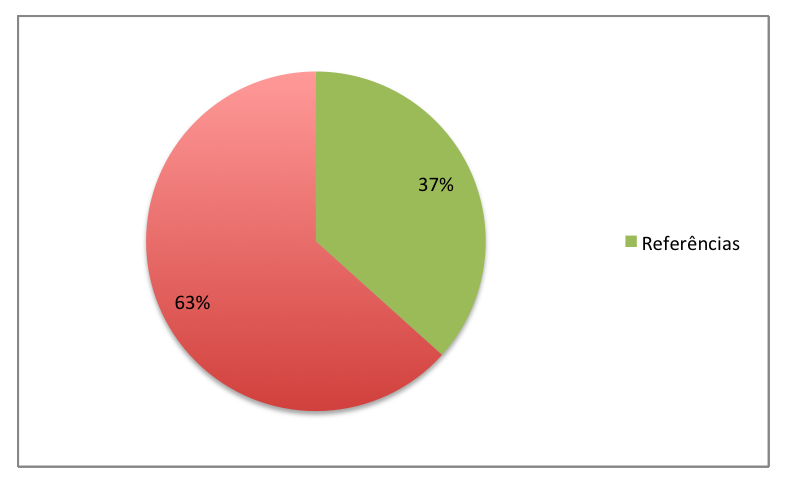
\includegraphics[width=0.8\textwidth]{capitulos/las/figuras/cultura.eps}}
	\caption{Percentual de trabalhos que referenciaram lições aprendidas da categoria ``Cultura organizacional"}
	\label{fig:cultura}
\end{figure}
